\documentclass[titlepage]{article}
\usepackage[document]{ragged2e}
\usepackage{amsmath}
\usepackage{graphicx}
\usepackage{indentfirst}
\usepackage{ragged2e}
\usepackage{tikz}
\usepackage{listings}
\usepackage{cite}
\usepackage{pdfpages}
\usepackage[font=it]{caption}
\usepackage{algorithm2e}
\usepackage{hyperref}

%\usepackage[a4paper, margin=1.5in]{geometry}

\RaggedRightParindent = 24pt
\linespread{1.3}


%set code style
\lstdefinestyle{default}
{
	language=C++,
	frame=single,
	tabsize=2,
	numbers=left,
	basicstyle=\scriptsize,
	showstringspaces=false,
	captionpos = b
}
%Set Algorithm style
\RestyleAlgo{boxed}
\LinesNumbered
\lstset{style=default}
%opening

\title{Modelling of Nanosecond time-scale Transient response of GaN LEDs \\ \textbf{Project Outline}}
\author{Zachary Humphreys}
\date{\centering ID: 200951438
	\\02/02/2018 \bigskip
\hrule \bigskip
A Thesis Submitted in partial fulfilment of the requirements for the degree of:\\
\textbf{Master of Physics} \\
Under the supervision of Dr. Joachim Rose \\
At the \\
\textbf{Department of Physics}
\bigskip

\includegraphics[scale=0.6]{LiverpoolLogo}
}


\begin{document}

\maketitle

\tableofcontents
\lstlistoflistings
\listoffigures
\listoftables
\listofalgorithms
\newpage

\section*{Declaration}
%\addcontentsline{toc}{Chapter}{Declaration}

I, Zachary Humphreys, hereby declare that this thesis is my own work and effort and that it has not been submitted anywhere for any award. Where other sources of information have been used, they have been acknowledged.
\bigskip \\
\hrule
\textit{Note: As this is the project outline, certain missing information, citations, and other incomplete sections will be labelled in \textbf{bold} font to bring attention to it.}
\hrule

\section{Abstract}
\begin{center}
In this thesis, the light emission properties of Gallium Nitride blue LEDs are modelled and explained, particularly of note being the unusual characteristics of one being switched on and off on nanosecond timescales. \\ Switching under these conditions require high voltages in both the forwards and reverse biases and effects that can normally be ignored appear to have much larger effects under these conditions and time scales. \\ Switching LEDs under these time-scales could be of particular use in the calibration of large photo-detectors which focus on detection of very small \textbf{approx\#ofphotons} bursts of photons (such as Neutrino detection experiments)\textbf{findcitationforsuperK}, and so require similarly small, but consistent amounts for calibration.
\end{center}



\section{History \& Introduction}
The very first semiconductor device was the photometer, developed by Von Siemens in 1875 \cite{G3Nsemicomp}(p6) (effectively a primitive solar cell) and hence, from the very inception of semiconductor devices, interaction with light has been closely related. However, it wasn't until 1907 until the electro-luminescence effect was discovered\cite{Sze}[p601] in the form of a point contact with a SiC substrate\cite{Sze}(p608) that emission of light, instead of absorption, was demonstrated. This electro-luminescence was different from radiative emission in both frequency and broadness of spectrum. But it wasn't for yet another 42 years, with the advent of the p-n junction in 1949, that the Light Emitting Diode (LED) as we know it today, was invented.\cite{Sze}(p608)\cite{G3Nsemicomp}(p1). \\
Unfortunately, due to them being made of Indirect Band-gap semiconductors, they had very poor efficiency, and it's progress remained stagnant with a lack of commercialisation\cite{G3Nsemicomp} until the discovery of direct band-gap designs of GaAs in 1962 which had a much higher Quantum Efficiency leading to the first semiconductor laser. Soon after, in 1964, indirect bandgap materials also improved with the process of "doping" (addition of impurities) being discovered.\cite{Sze}(p608) \\
Up until this point, all the discovered LED technology had led to LEDs with spectra in the Infrared to the lower frequency end of the visible spectrum and in 1971, Pankove et. al. reported the first GaN LED and hence, the first LEDs with frequencies in the blue to UV range. \cite{NSD}(p3) However, traditional methods growing crystals of this nature were difficult and would lead to progress in a different technique: Epitaxial growth, where a film of crystal is grown from the surface of another.\cite{G3Nsemicomp}(p8)\cite{Nakamura}(p4). The only problem was, all of the known materials that would produce blue light had short-comings. Of note, was the epitaxial growth of GaN had a lattice mismatch to its best substrate (Sapphire) of 13.8\% , compared with ZnSe (an alternative) on GaAs with a 0.3\% mismatch and could thus easily be grown with few defects, leading to high quality crystals.\cite{G3Nsemicomp}(p11,13)\cite{Nakamura}(p4). \\
These films were generally deposited by either Molecular beam, or metalorganic vapour phase Epotaxy (MOVPE) but would require temperatures of $\approx1300$K and high pressures. As a result of the high rate of defects in GaN at the time ($10^9cm^{-2}$) made ZnSe generally the more popular choice for scientists ($10^3cm^{-2}$) which in turn, led to little research in the area.\cite{Nakamura}\\
In 1990, Nakamura developed a technique (low carrier gas flow MOCVD) for producing high quality, uniform GaN using ammonia, but there was still the challenge of successfully doping it, meaning overcoming Mg acceptor dopant producing complexes with the H \cite{Nakamura}(p5) and finding a suitable Donor n-type. The first GaN pn junction was created in 1991 with an output power of $42\mu W$ and a External Quantum Efficiency of 0.18\% at a wavelength of 430nm (far lower than the minimum 1mW for usefulness.) \\
Only after the discovery of InGaN, and its ideal properties as an active layer in a Double Heterostructure (DH), where it's bandgap was able to be tightly controlled through level of doping with tight control was the first Blue DH LED created, in 1993 which\cite{Nakamura}(p7), in turn, would lead to the first white LED with the addition of a white-phosphor\cite{Sze}(p608), \\The highest External Quantum efficiencies for LEDs are being achieved by GaInP encased in epoxy with 55\%,\cite{EQE} a massive improvement from the earliest versions of LEDs. In comparison, an oil lamp produces approximately $0.1lmW^{-1}$, an incandesceent bulb produces  $16lmW^{-1}$, fluorescent  $70lmW^{-1}$, but an LED will produce  $300lmW^{-1}$\cite{Nakamura}(p3) and the very first pn junction laser diode in visible spectrum of  $\approx 0.1lmW^{-1}$ created by Holonyak in 1962. \cite{Kittel}(p580)\\
Due to their high efficiency and ability to be tightly controlled, LEDs have been implemented in many technologies from simple indicator lights, to room illumination, but recently, they've been considered for calibration of Large photo-detection experiments such as Hyper-K and ANTARES neutrino detection experiments, where they aim to detect the Cherenkov radiation from Muon's produced by neutrinos interacting with matter. These interaction create very short pulses of very few photons of approximately blue colour, and thus, a similar pulse of light would be preferable to calibrate such an experiment.\textbf{CITATIONS NEEDED} \\
For this, the use of Blue, GaN-based LEDs pulsed at nano-second time-scales has been proposed. However, as the lifetime of charge carriers in these materials is on the order of nanoseconds for InGaN/AlGaN DH LEDs\cite{Brailovsky}, it has generally been considered practically impossible to produce such results, and conventional methods for driving LEDs result in rather low switching frequencies on the order of 1GHz. \\ To the contrary, it has been demonstrated that such pulses can be achieved experimentally \textbf{Rose citation?} and thus, an investigation into the mechanism will be conducted as the objective of this thesis, and whether experimental results can be simulated with current models and understanding.


\section{Background Physics and Past Work}
\subsection{Fundamentals}
At the core of this investigation are the physics of charge-carrier transport within semiconductors, and semiconductor junctions.\\
The simplest type of junction is the p-n, which made of a single crystal of semiconductor, doped with impurities to produce regions with different "majority carries". Donor atoms, which have more valence electrons than the intrinsic semiconductor, when infused into the semiconductor, result in an \textit{n-type} region with a majority carrier of electrons.\cite{Kittel}(p570) When these impurities become ionized by depletion of the carriers, an electric field is generated internally.\cite{Sze}(p16) \textit{P-type} semiconductor is produced in much the same way, but with doping with atoms with fewer valence electrons ("acceptor" impurities), leaving "holes" which become the majority carriers in that region, which are simply absences of an electron compared to the intrinsic lattice. These holes act as if they were  positive charges when subject to electric and magnetic fields and have the equivalent equations of motion.\cite{Kittel}(p206-8)\\
By having a region of \textit{n-type} and \textit{p-type} semiconductor in contact, a p-n junction is formed, and the excess majority carriers from each attempt to diffuse to produce uniformity across the device, leading to the two majority carriers recombining at the interface to cancel each other out, leaving ionization of the impurities in both regions. The electric fields generated leads to potential barrier preventing complete diffusion and leads to separation of remaining electrons holes, and a depletion region near the potential barrier.\cite{Sze}(p80)\\
The understanding of the movement of these charge carriers is what is needed to understand the nature of this fast-switching of an LED.\\
As described above, carriers respond to electric fields. An application of an electric field, or magnetic field, will impart a Lorentz force
\begin{equation}
\vec{F} = q(\vec{E}+\vec{v}\times\vec{B})
\end{equation}
upon these particles, which will lead to an overall Drift current, $\vec{J}_{drift}$. With the addition of the current from the diffusion of these carriers in concentration gradient, $\vec{J}_{dif}$, we find the most widely used approximation to describe carrier transport in semi-conductors:\cite{SzeHiSpeed}(p58)
\begin{eqnarray}
&\vec{J}_{tot} = \vec{J}_{drift} + \vec{J}_{dif}\\
&\vec{J_n} = q(n\mu\vec{E} + D\nabla n)
\end{eqnarray}
for electrons, where $\vec{J_n}$ is the current density vector, $q$ is the charge on the electron, $n$ is the charge density of electrons, $\mu$ is a mobility constant, $\vec{E}$ is the applied electric field, and $D$ is the drift mobility constant, which in a non-degenerate case [in which the doping concentration $N_D$ is $\ll N_C$ than the Number of conduction band states, and hence obey Boltzmann statistics\cite{Sze}(p18)] has the Einstein relation:\cite{SzeHiSpeed}(p58)
\begin{equation}
D = \frac{k_B T}{q}\mu
\end{equation}
where $k_B$ is the Boltzmann constant, and $T$ is temperature. \\
This drift-diffusion equation can be modified to also account for conduction band energy $E_C$, as well as position dependence through effective mass $m*$ [which results from the parabolic energy-band equation $E(k) = \frac{\hbar^2k^2}{2m*}$\cite{Sze}(p13)] resulting in:\cite{Frensley}(p21)
\begin{equation}
J_n = -q\mu_n n \nabla V + \mu_n n \nabla E_C + q D_n \nabla n - \frac{3}{2}qD_n n \nabla \ln(m*_C)
\end{equation}
These current equations come are joined by two other equations of importance: Maxwell's equations (specifically Poisson's equation):
\begin{equation}
\nabla \vec{E} = \frac{\rho(x,y,z)}{\epsilon}
\end{equation}
(where $\rho$ is the charge density, and $\epsilon$ is permittivity) and the continuity equation for time-dependent systems:
\begin{equation}
\dfrac{\partial n}{\partial t} = G_n - R_n + \frac{1}{q}\nabla\cdot\vec{J}_n
\end{equation}
In which $G_n$ and $R_n$ are thermal generation and recombination rates respectively.\cite{Sze}(p63)\cite{NSD}(p287)
\medskip
An alternative to this method of modelling transport within the device, is through the semi-classical Boltzmann Transport equation (BTE), describing the movement of the charge carriers through phase space, and in bulk material has the form:
\begin{equation}
\Big(\dfrac{\partial f(\vec{r},\vec{k},t)}{\partial t}\Big)_C = \dfrac{\partial f(\vec{r},\vec{k},t)}{\partial t} + \vec{v}\cdot\nabla f(\vec{r},\vec{k},t) + \frac{E}{\hbar}\cdot\nabla_k f(\vec{r},\vec{k},t)
\end{equation}
Where $\vec{r}$ and $\vec{k}$ are position and phase-space vectors respectively, and $f(\vec{r},\vec{k},t)$ is the particle distribution function.\cite{NSD}(p70)\\
The evolution of this particle distribution function in time is handled through scattering of these electrons and holes treated as classical point particles:
\begin{eqnarray}
\Big(\dfrac{\partial f(\vec{r},\vec{k},t)}{\partial t}\Big)_C & = \int\{f(\vec{r},\vec{k}',t)[1-f(\vec{r},\vec{k},t)]S(\vec{k}',\vec{k})\\
&-f(\vec{r},\vec{k},t)[1-f(\vec{r},\vec{k}',t)]S(\vec{k},\vec{k}')\}d\vec{k}'
\end{eqnarray}
Where $S(\vec{k},\vec{k}')$ is the complete set of scattering rates from $\vec{k}$ to $\vec{k}'$. This scattering rate comprises of many terms, incorporating scattering due to Polar optical phonons, acoustic phonons, impurities, and non-parabolic band scattering amongst others.\cite{NSD}(p72-6)\\
Due to it being less popular than the Drift-Diffusion model, this method was not explored in much depth.\\
In the search for existing literature on the topic of nanosecond time-scale physics for LEDs, two papers of note were encountered which modelled LEDs under these conditions. The following subsections detail these two existing pieces of literature.
\subsection{Existing Literature: Windisch}
In the paper, \textit{“Large-Signal-Modulation of High-EfficiencyLight-Emitting Diodes for Optical Communication”}, R. Windisch, et. Al\cite{Windisch} produced a model to explain the rapid recombination that happened up to a factor of two-times faster than the radiative recombination lifetime which, in general, is given by:
\begin{equation}
\tau_{rec} = \dfrac{n}{R_{rec}}
\end{equation}
where $R_{rec}$ is the radiative recombination rate, which in this case, is given by:\footnote{This is not the only form found in literature for $R_{rad}$. Alternatives include:$R_{rad} = Bnp \cdot \Big[1-\exp(-\frac{F_n-F_p}{k_B T})$ \cite{NSD}(p306) which includes Quasi-Fermi level dependancy, and $R_{rad} = B(np-n_0 p_0)$\cite{NSD}(p289).}
\begin{eqnarray}
R_{rec} = Bn(p_0 + n)\\
p = p_0 + n
\end{eqnarray}
where B is the radiative recombination constant, which is found experimentally,\cite{Windisch}(p2) and $p_0$ is the doping concentration.\\
In this model, a number of assumptions were made: The model was based on a Double Heterostructure LED (one where two semiconductors materials are grown together, where the different semiconductors have different band-gaps in a "sandwich" like arrangement.\cite{Sze}(p56)), had instant voltage and current switching, and had negligible recombination through means other than radiative.\\
The boundary condition was set so at $t = 0$, $n = 0$, and increased in time following:
\begin{equation}
\dfrac{dn}{dt} = R_{in}(t) - R_{rec}(t)
\end{equation}
Where $R_{in}$ was simply the injection rate in, defined as:
\begin{equation}
R_{in} = \frac{J}{qw}
\end{equation}
Where $w$ was the width of the active region of the device. From this, an analytical solution for the carrier density was found:\cite{Windisch}(p2,3)
\begin{eqnarray}
&n(t) = -\frac{p_0}{2} + \frac{\omega}{2B} \tanh(\frac{\omega}{2}(t+C))\\
&\omega = \sqrt{B^2p_0^2+4\frac{JB}{qw}}\\
&C = \frac{2}{\omega} arctanh(\frac{p_0 B}{\omega})
\end{eqnarray}
and found that in the cases that the active region is highly doped, the device does indeed follow the expected Recombination lifetime exactly, but that in the case of low doping, where injected carrier concentration isn't proportionally negligible, the switch time can up to a factor of two faster.\cite{Windisch}(p4)\\
However, this paper neglected the fact the carriers have charge and the associated Electric fields they'd generate, and focused exclusively on the active region of the device for simplicity.
\subsection{Existing Literature: Brailovsky \& Mitin}
The second paper of note was \textit{Fast switching of light-emitting diodes} by A.B. Brailovsky, and V.V.Mitin\cite{Brailovsky} where the authors produce an analytical model roughly based on the Drift-Diffusion equation. Again, like the previous paper, it assumes step-like instant-switching of the voltage.\\
The basis of the model is that switching speed may be increased by switching from direct current pumping to controlling the voltage  across the LED.\cite{Brailovsky}(p2) By starting with the equation for change in electron concentration around the p-region of the device:
\begin{equation}
\dfrac{\partial n}{\partial t} = D \dfrac{\partial^2n}{\partial t^2} - \frac{n}{\tau}
\end{equation}
where $D$ is the diffusion coefficient, and $\tau$ is the recombination lifetime of the electrons in the p-region. After moving to dimensionless variables, setting the boundary conditions for $n(x,t)$ of $n(0,0) = 0$, $n(0,t) = \Delta n(1-\exp(-\alpha t))$, and $n(\infty,t) = 0$, then applying a laplace transformation, a solution was found of:
\begin{equation}
n_p(x) = \Delta n e^{-x\sqrt{p+1}}\Big[\frac{1}{p}-\frac{1}{p+\alpha}\Big]
\end{equation}
where $\alpha$ is a constant determining how fast concentration at the junction changes, and $n_p(x)$ is the Laplace transform of $n(x,t)$.\cite{Brailovsky}(p2) This applies to the switching on of the device, and not to the switching off, and also isn't complete, as it ignores the Electric fields effects like the previous paper and neglects the drift effects in this solution.\cite{Brailovsky}(p3) \\
From this solution, it was shown that the current in the device in the case of large values of $\alpha$ ($\approx>10$) resulted in large reverse currents within the device, which could be the reason for switching times faster than the Radiative Recombination lifetime.\\\cite{Brailovsky}(p2)
\section{Method}\label{sec:Method}
In order to explore the behaviour of the light emitting diode at short time-scales, two simulations were created to explore how different interpretations of the device would affect the results: A "macroscopic" simulation treating the device as a singular object, and a second "microscopic" simulation that took into account of internals of the device. The theoretical foundation for carrier transport in both device simulations was the Drift-Diffusion model due to its common usage, and simpler implementation than competing models, such as the Semi-classical Boltzmann Transport Equations that has its basis in the scattering of classical point-like holes and electrons from one set of phase-space coordinates to another.\cite{NSD}[p70-6] \\
The goal of both simulations was to produce plots of the full width half maximum ($\sigma_{FWHM}$) as a function of the number of photons in the pulse, to compare with the real device output.\\
Experimentally, voltage across the diode was ramped up and down over the period of several nanoseconds, with the forwards bias injecting charges, and the reverse bias pulling any remaining charges that hadn't combined, out of the device. In both models, to match the experimental conditions, the applied voltage to the diode was modelled as a tent map with the equations:
\begin{eqnarray}
	V(t) = \begin{cases}
	\alpha t &t < t_{trans}\\
	\alpha(2t_{trans} - t) &t \geq t_{trans}\\
	\end{cases}
\end{eqnarray}
where $V$ is the bias voltage, $t$ is the time, $t_{trans}$ is the transition time from voltage ramp up to voltage ramp down, and $\alpha$ is the voltage ramp scale (found experimentally to be $4Vns^{-1}$). This is an approximation to the experiment as it is not possible to switch instantly from forwards to backwards, with a more realistic model expecting some rounding to the graph graph during switching on, and switching from forwards to backwards. 
\begin{figure}[t]
	\hrule
	\centering
	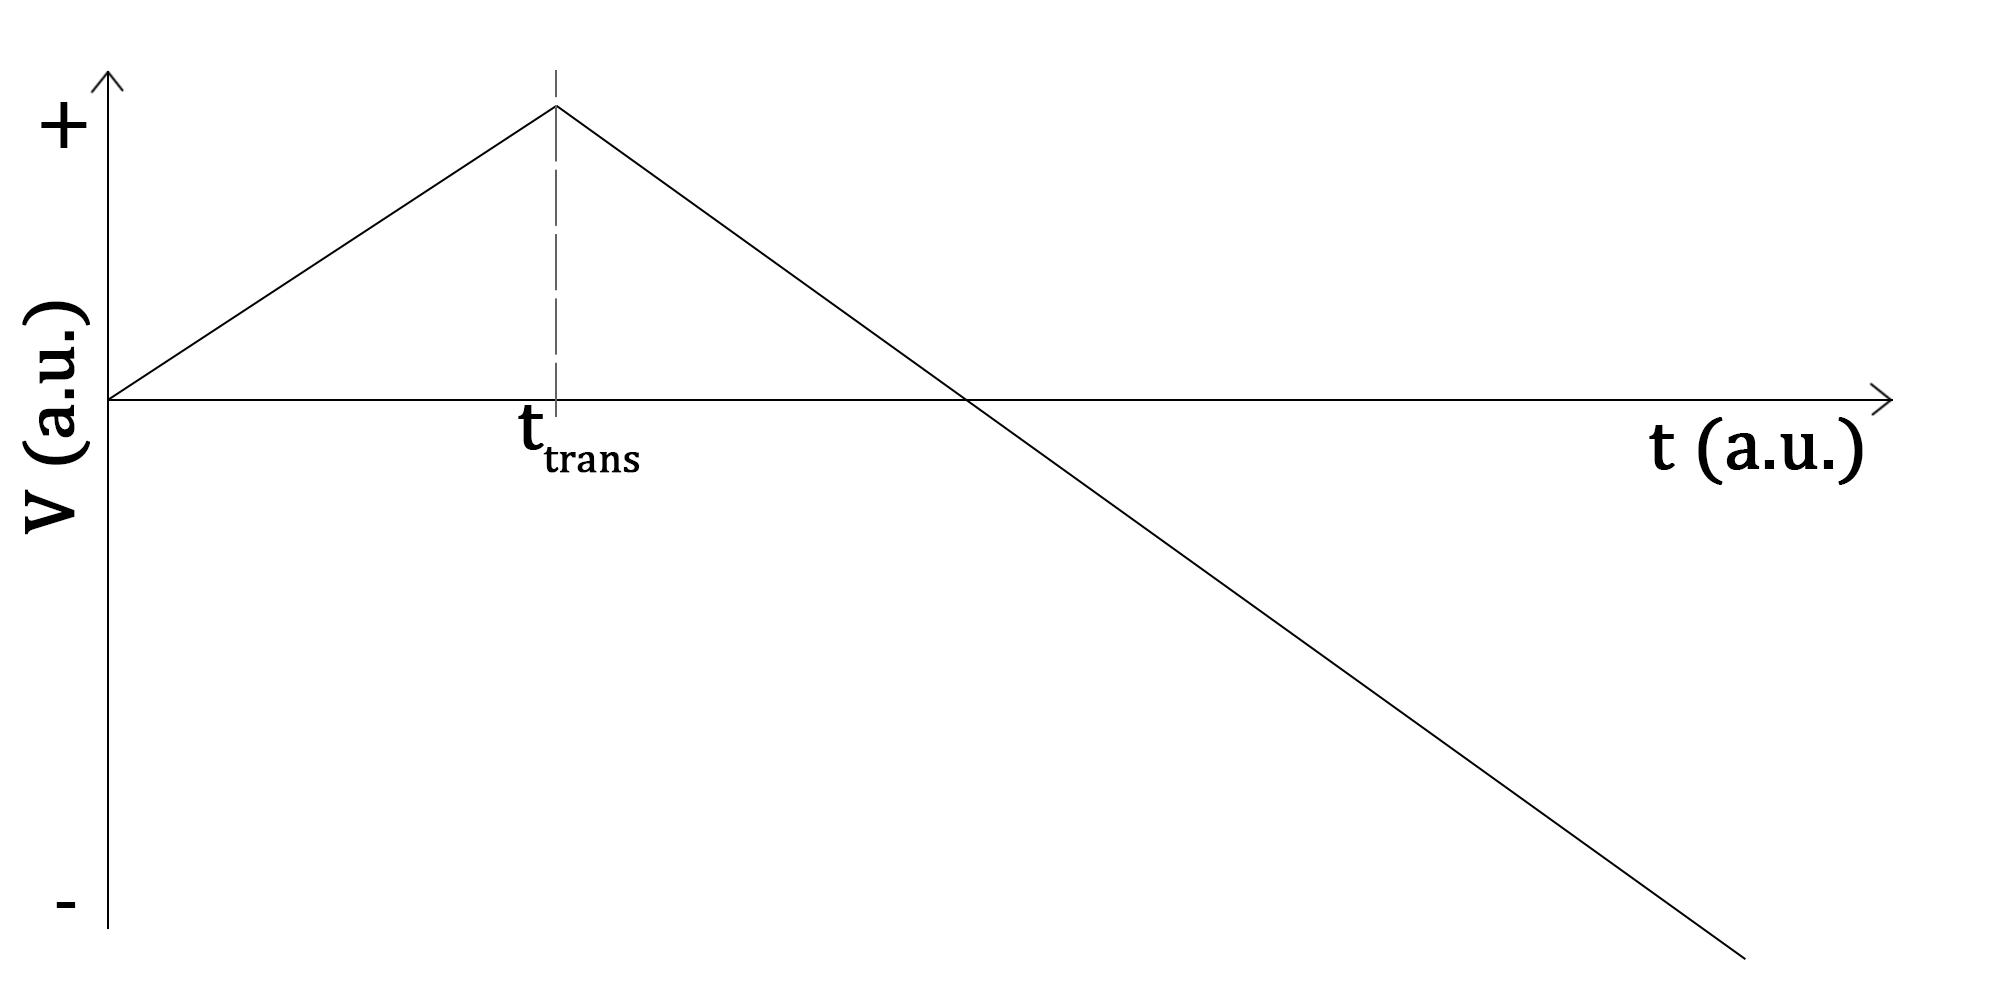
\includegraphics[scale=0.12]{Figures/V_tent}
	\caption{\label{graph:V_tent}Graph of the approximate shape of the voltage ramp up and down used experimentally.}
	\hrule
\end{figure}
\subsection{"Macroscopic" Model}
\subsubsection{Conceptual Overview}
\begin{figure}[t]
	\hrule
	\centering
	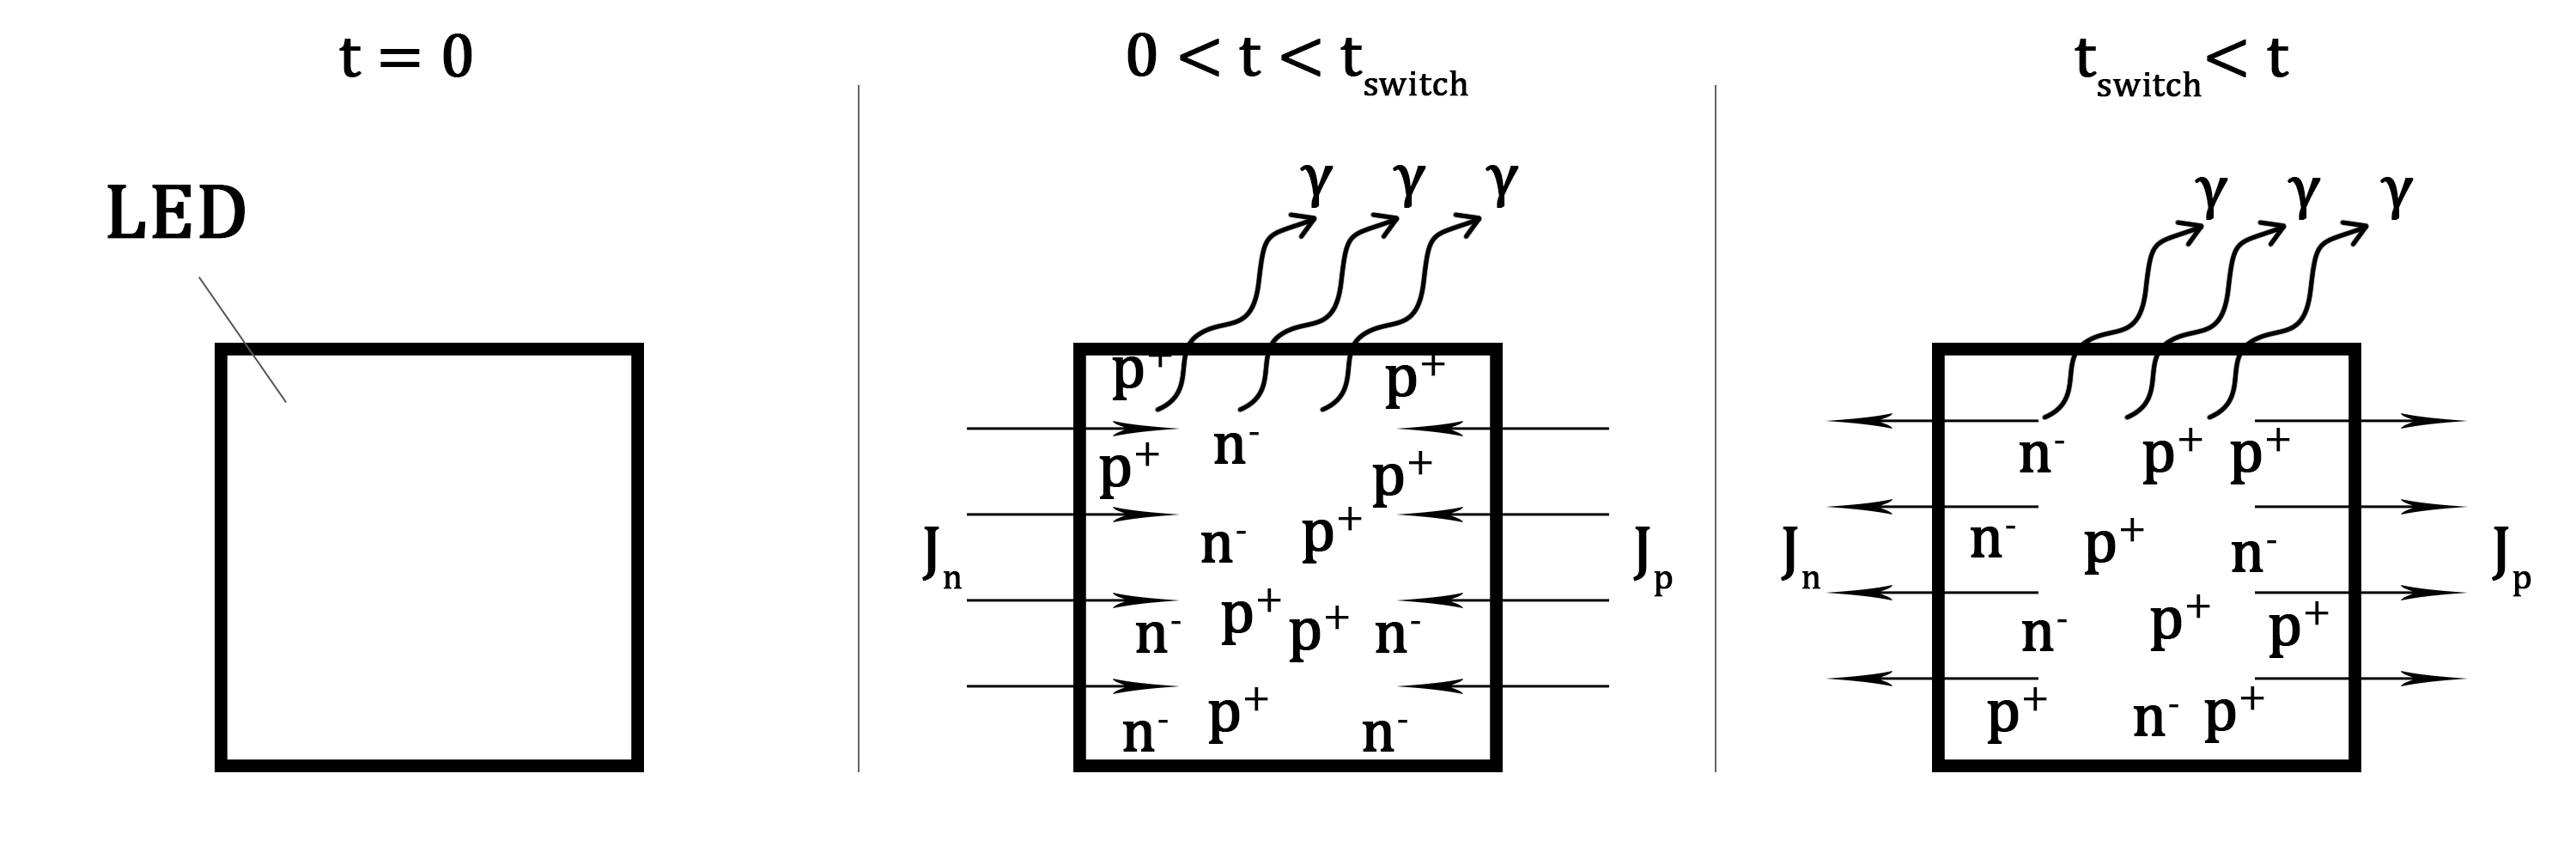
\includegraphics[scale=0.12]{Figures/Bucket_overview}
	\caption{\label{fig:bucketOverview}This figure displays the concept behind the macroscopic model where after time, $t=0$, electrons and holes ($n^-$ and $p^+$ respectively) are injected by currents $J_n$ and $J_p$ until the switch time, where upon the currents are reversed until all the charges have either combined to create photons ($\gamma$), or have been removed.}
	\hrule
\end{figure}
In this simulation, the device was modelled as a single, complete object where charges would be injected, and photons ejected as a result of holes and electrons in the device combining (fig.\ref{fig:bucketOverview}). This interpretation would be similar to treating the device to that of a leaky capacitor under Direct Current operation. This is a not-entirely unrealistic as "real" LEDs do have some small level of capacitance in the form of charge storage and  depletion layer capacitance.\textbf{[CITE: VALEDAR,p30]} This model also means that opposite charges can interact immediately once inside, as the device is treated as so small that the charges are injected in the same place.\\
\subsubsection{Calculating number of charges}
The core calculation for number of charges in the device was done in a discrete time-step manner thus:
\begin{eqnarray}
&n(t) &= n(t-1) + \dfrac{dn}{dt}\Big|_{n=n(t)} \\
\hookrightarrow &n(t) &= n(t-1) + n_J(t) - n_R(t) 
\end{eqnarray}
where $n(t)$ is the number of charges at time t, $n_J(t)$ is number of charges injected at time t, and $n_R(t)$ is the number of charges recombined at time t, with the boundary conditions, $n(0), n(t_{end}) = 0$ with the approximation that Thermal Generation and Recombination were negligible.\\
As both negative and positive charges would be injected at the same rate in this model, it is convenient to work in just one of them (in this case, negative) to simplify certain calculations.\\
To calculate the number of injected charges, the approximation was taken that the LED itself was an Ohmic device, with resistance of $5\Omega$, and using Ohms law:
\begin{eqnarray}
	&I =& \dfrac{V}{R} =  \dfrac{q n_J}{t}\\
\hookrightarrow	&n_J =& \dfrac{V}{qR}t
\end{eqnarray}
where $V$ is the external applied Voltage, $R$ is the resistance, $q$ is the charge on the electron, and $t$ is the amount of time the current is being applied for.\\
The number of charges lost to Radiative Recombination can be found from the  Radiative recombination rate equation given by:\cite{NSD}[p289,306]\cite{Sze}[p614]
\begin{eqnarray}
&R_{rad} =& Bnp\\
\hookrightarrow &R_{rad} =& Bn^2\Big|_{p=n} = n_R 
\end{eqnarray}
where $B$ is the bulk recombination rate constant.\\
\subsubsection{Simulation Algorithms}
The method for finding the number of photons, and FWHM of the associated pulse, was done by running the device simulation over a range of transition times, incrementing the transition time by a small step each loop:\\
\begin{algorithm}[H]
	Create arrays to store FWHM and Number of photons\; 
	\For{$t_{trans} = 0$ to $t_{trans-max}$}
	{
		Carry out the simulation at $t_{trans}$\;
		Save the resulting FWHM and Number of photons to arrays\;
	}
	Print the arrays to file\;
	\caption{Macroscopic outer loop \label{alg:Mac:outer}}
\end{algorithm}
\bigskip
In the program, the size of the transition step, the maximum transition step, and the simulation step can all be determined at run-time via console input at the start.\\
The algorithm for the nested simulation step of the outer loop is defined by Algorithm \ref{alg:Mac:inner}.\\
\begin{algorithm}[H]
	Create array for number of photons and current time\;
	Create Cumulative Radiation variable and set to 0\;
	\While{$n \geq 0$}
	{
		Increment simulation at $t$ by $t_step$\;
		Add time onto end of the time array\;
		Find V at $t$ from tent map\;
		Find $n_J$ from V \;
		Add $n_J$ to $n$\;
		Find $n_R$ (and hence number of photons)\;
		Take $n_R$ from $n$\;
		Add $n_R$ onto end of photon array\;
		Add $n_R$ to cumulative photons.\;
	}
	Use arrays to find FWHM\;
	Send total photons and FWHM to outer loop.\;
	\caption{Macroscopic Inner simulation loop \label{alg:Mac:inner}}
\end{algorithm}
\bigskip
From both of these algorithms, it's clear that the smaller the time step for both the transition time and inner simulation time, the higher the resolution of the data, so generally, the step for the simulation was on the order of $10^{-3}$ times the transition time.\\
To find the FWHM of the pulse, Algorithm \ref{alg:Mac:FWHM} was used. From this method, the error on the FWHM is no more than the width of two bins.\\
\begin{algorithm}[H]
	Find peak photon count bin in the photon array\;
	Find first bin to fall below half this value before and after peak bin\;
	Use bin numbers to find associated times in the time array\;
	Subtract the time from the after-peak bin from the before-peak bin\;
\caption{Finding photon Pulse Full Width Half Maximum \label{alg:Mac:FWHM}}
\end{algorithm}
\bigskip
The resulting data generated by this simulation was then outputted to a .csv file where it could be analysed.

\subsection{"Microscopic" Model}
\subsubsection{Conceptual Overview}
This model was produced to compare the results with the Macroscopic interpretation of the device. It centred around numerically solving the charge Continuity Equations through calculating both the Drift-Diffusion and Poisson's equations:\cite{Frensley}[p21]
\begin{eqnarray}
	&J_n = -q\mu_n n\nabla V + \mu_n n \nabla E_c + q D_n \nabla n\\
	&J_p = -q\mu_p p\nabla V + \mu_p p \nabla E_v - q D_p \nabla p\\
	&\nabla\cdot\vec{D} = \rho
\end{eqnarray}
where the first and second equations are the drift-diffusion equations with the addition the second terms to account for spacial variation of band structure, and the third equation is Gauss' law.\\ 
This was done by dividing the device into segments. A visual representation can be found in Figure \ref{fig:Mic:Segment}.\\
\begin{figure}
	\centering
	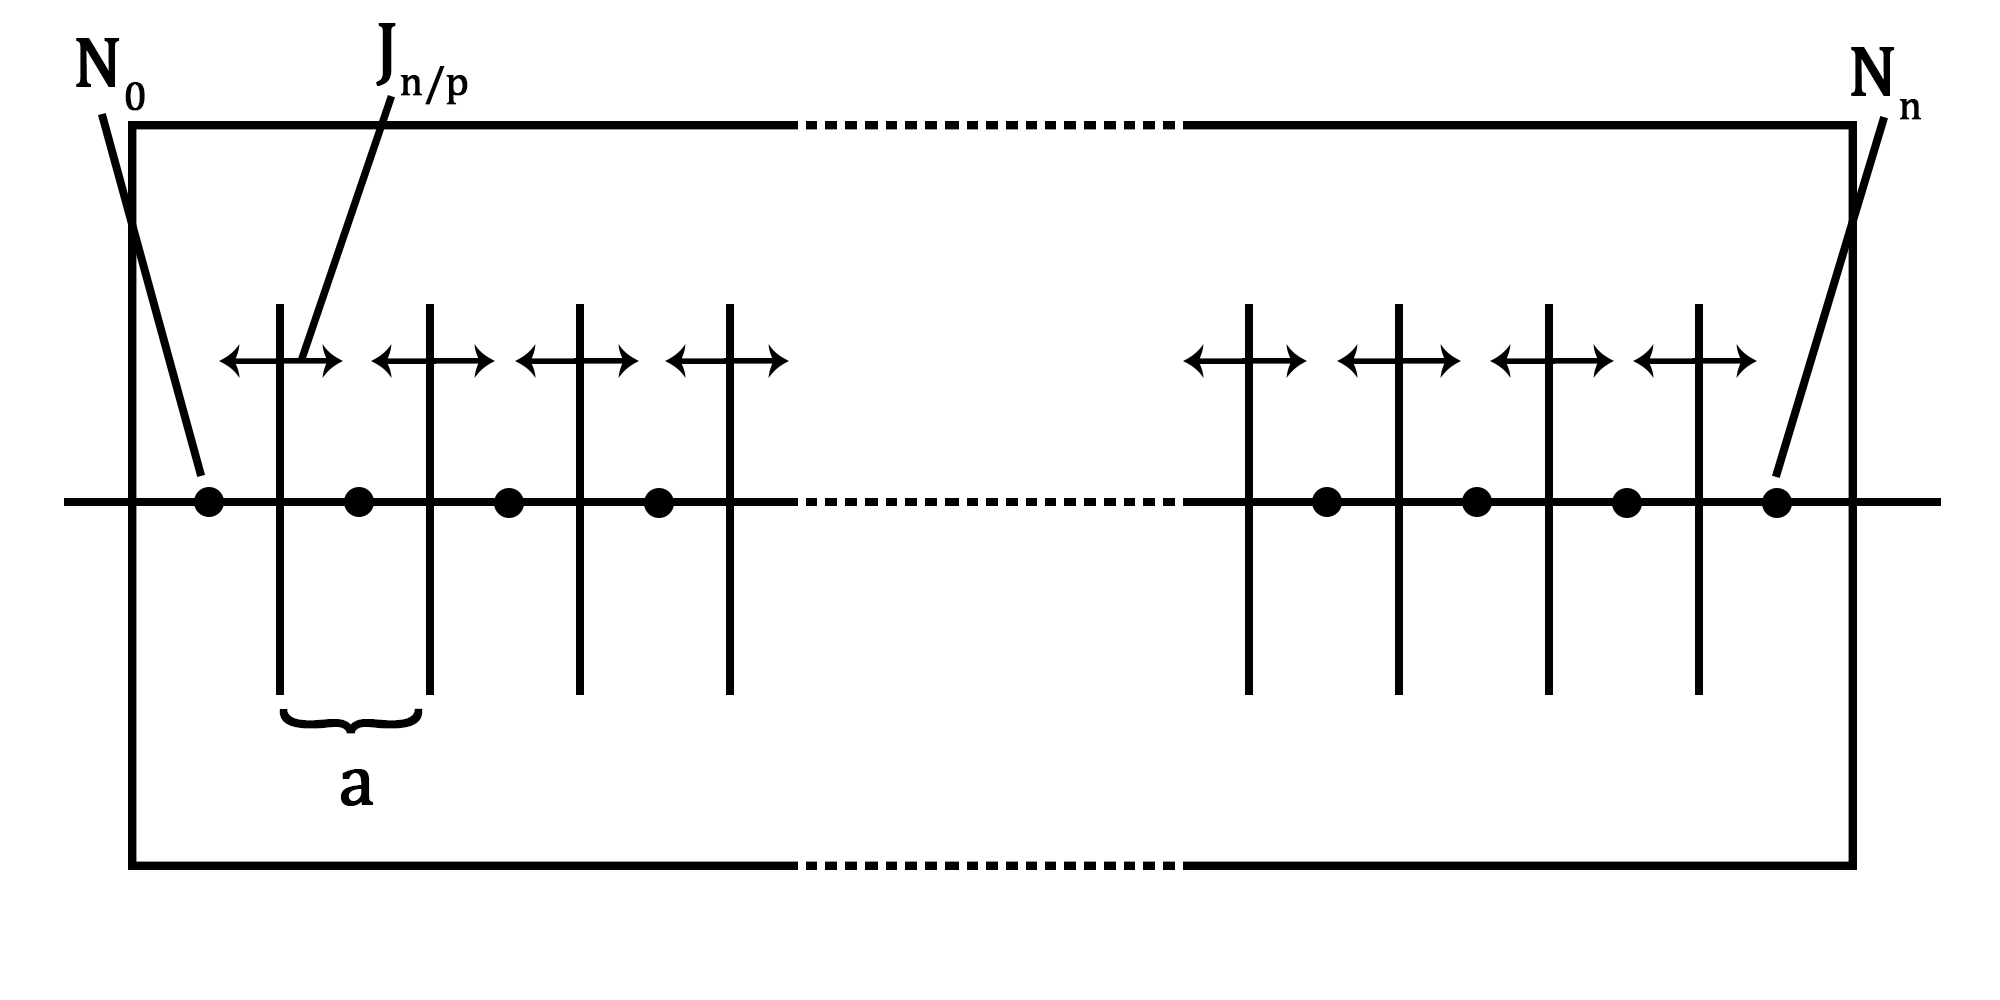
\includegraphics[scale=0.15]{Figures/Segmented}
	\caption{\label{fig:Mic:Segment}Visual representation of Microscopic model's segmented device. $N_x$ is node at position x, $a$ is the node width, and $J_{n/p}$ is the current density between two nodes for either electrons($n$), or holes($p$).}
	\hrule
\end{figure}
Each "node" along the device has a set width, $a$, and contain several variables and constants: The charge densities for electrons and holes ($n$ and $p$ respectively), and the potential at that point $V$ being the variables, and with constants determining doping of acceptor atoms $N_a$, doping of donor atoms $N_d$, and the Conduction and valence band relative energies, $E_c$ and $E_v$ respectively. \\
The device would be constructed as a "string" of these Nodes, with a set length, and area perpendicular to the current, which would limit it strictly to cuboid shaped devices. \\
Due the increased complexity of this model, there are more initial conditions to be considered, such as how many nodes there are, the specifications of each of the nodes, the overall dimensions and parameters of the device, etc. so the program running this simulation was designed to have similarly broad functionality. A command-line interface was built to allow a user to do the following tasks: load and save a "device" to file, bring a device to equillibrium, run the simulation on a device for a set of conditions, and run the a range of simulations for a range of conditions to calculate a range of photon pulses for different transition times to find the how the FWHM varied with number of photons in a pulse. \\
\subsubsection{Converting the equations to numerical form}\label{sec:Meth:Mic:eqn}
In order to do calculation using the Drift-Diffusion and Poisson's equations, they first had to be discretised. This could be achieved through the use of Taylor expansion's.\cite{Nkonga}\cite{ECE606}\\
Using the Taylor expansions of:
\begin{eqnarray}
	f(x+\delta x) &= f(x) + \delta x\dfrac{df}{dx}\Big|_{x = x+\delta x} + (\delta x)^2 \dfrac{d^2f}{dx^2}\Big|_{x = x+\delta x} + ...\\
	f(x-\delta x) &= f(x) - \delta x\dfrac{df}{dx}\Big|_{x = x-\delta x} + (\delta x)^2 \dfrac{d^2f}{dx^2}\Big|_{x = x-\delta x} - ...\\
\end{eqnarray}
it was possible to find approximations for both first a second derivatives by using:
\begin{eqnarray}
	\dfrac{df}{dx}\Big|_{x+\delta x/2} =& \frac{f(x+\delta x)-f(x-\delta x)}{\delta x}\\
	\dfrac{d^2f}{dx^2}\Big|_{x_i} =&  \dfrac{f(x+\delta x) + f(x-\delta x) - 2f(x_i)}{(\delta x)^2} 
\end{eqnarray}
Using these approximations, it was possible use Gauss' law to find the potential at each node point using:\cite{ECE606}
\begin{eqnarray}
	&\nabla\cdot\vec{D} = \rho \\
	&\nabla^2 \cdot V = \dfrac{\rho}{\epsilon_r \epsilon_0} \\
	&\nabla^2 \cdot V = \dfrac{V_{i+1}+V_{i-1}-2V_i}{a^2} \\
	\hookrightarrow & \dfrac{V_{i+1}+V_{i-1}-2V_i}{a^2} = \dfrac{\rho}{\epsilon_r \epsilon_0}\\
	& \dfrac{V_{i+1}+V_{i-1}-2V_i}{a^2} = \dfrac{q}{\epsilon_r \epsilon_0}(p+N_D-n-N_A)
\end{eqnarray}
Where $i$ indicates the node index. Using the same method, current densities $J_n$ and $J_p$ can be calculated thus:
\begin{eqnarray}
	J_n =& -q\mu_n(\dfrac{n_{i+1}+n_{i}}{2})(\dfrac{V_{i+1}-V_{i}}{a})\\
	 +& \mu_n (\dfrac{n_{i+1}+n_{i}}{2})(\dfrac{E_{c(i+1)}-E_{c(i)}}{a}) + qD_n(\dfrac{n_{i+1}-n_{i}}{a}) \\
	J_p =& -q\mu_p(\dfrac{p_{i+1}+p_{i}}{2})(\dfrac{V_{i+1}-V_{i}}{a})\\
	 +& \mu_p (\dfrac{p_{i+1}+p_{i}}{2})(\dfrac{E_{v(i+1)}-E_{v(i)}}{a}) - qD_p(\dfrac{p_{i+1}-p_{i}}{a}) \\
\end{eqnarray}
These three equations form the basis for the equilibrium and simulation abilities of the program.
\subsubsection{Program functionality: Saving \& Loading}
To allow use of user defined devices in the simulation process, a method of inputting the data rather than having it hard coded was necessary. To achieve this, a loading and saving method was designed.\\
A specific \textit{.csv} file format was developed that could be read by the program. An overview of the specifics of the format can be found in the \textbf{APPENDIX: TODO} to allow for the reader to create their own. This file would contain all the necessary information to create a device in the program, including: device length, area, resistance, number of nodes, and each of the individual node's data. To enable ease of reading for the program, a second internal file-type was created based on this file called a "doesn't include commas" file that was, in essence, this specifically structured .csv file type with all commas removed. This .dic file was easier to read and less error prone on reading, and would be automatically generated by the program.\\
The program could also save the current device in memory to a .csv file in the correct format to be transported, permanently recorded, or opened in an external spreadsheet or text editor program. This makes editing or altering device data far easier for the user.
\subsubsection{Program functionality: Equillibrium}\label{sec:Mic:Eqm}
Once a device has been loaded into the program, the user is able to bring the device to "equilibrium". This is done by running the continuity equation simulation on the device with no external input until a minimum total internal current is reached (defined by the user, recommended $\approx 1cm^{-3}s^{-1}$ or less) where total internal current is defined by:
\begin{eqnarray}
	&J_{tot} = \sum\limits_{i=1}^{n}J_i\\
	&J_i = J_{n(i)}+J_{p(i)}
\end{eqnarray}
 This step is important to ensure the calculations have the intended behaviour and that running a simulation cycle doesn't result in excess photons being released from the device not already being in steady-state equilibrium. The following algorithm was used to achieve this:
\begin{algorithm}
	\While{$J_{tot} < tolerance$}
	{
		Calculate V at each node\;
		Calculate $J_n$ between each node and transfer charge density\;
		Calculate $J_p$ between each node and transfer charge density\;
		Cancel any charges that would recombine\;
		$J_{tot} = \sum J_{n(i)}+J_{p(i)}$
	}
\caption{\label{alg:mic:Eqm}Algorithm for bringed device to equillibrium}
\end{algorithm}
As running this algorithm at standard $J$ values would be very slow, a user-defined "Approximation" multiplier is used to speed this process up (typically a value from $10^3$ to $10^6$ is recommended.) This multiplier simply takes what the exchange current $J$ would be, and multiplies it by this value. Very large values has undefined behaviour, and in such cases, reloading the device from file is necessary, but without it, this process could take many millions of iterations. \\
Though not used in the final program, the code has debug functionality to print device status to file and console whilst this is happening, as well as print $J_tot$ to file for each iteration.

\subsubsection{Program functionality: Single simulation}
Using many of the same principles as the "Macroscopic" device model program and its algorithms, this command takes the device loaded and injects charges following the voltage tent map, and Ohmic D.C. modelling. It uses exactly the same code for finding FWHM of the pulse, though due to fundamental differences in design, the algorithms for finding the number of photons released from recombination are slightly different.\\
From device equilibrium where:
\begin{eqnarray}
	&n_R(t=0) = 0\\
	&J_{tot}(t=0) \approx 0\\
	\hookrightarrow &\dfrac{dn}{dt}\Big|_{t=0} \approx 0
\end{eqnarray}
and same for holes, injection of electrons from one end and holes from the other can begin.\\
This is done in the same time-step like manner of the Macroscopic device, however the algorithm is adjusted to:\\
\begin{algorithm}[H]
	\While{$n_R \geq 0$}
	{
		Add $t_step$ to $t$\;
		Find V at $t$\;
		Find $J_{input}$ from V\;
		Find $V_i$ for each node\;
		Propagate $n$ and $p$ through device with $J_n$ and $J_p$\;
		Find $n_R$ at each node and remove respective charge densities\;
		Save $n_R$ to histogram bin arrays\;
		Save respective $t$ to corresponding array\;
	}
	Find FWHM using Algorithm \ref{alg:Mac:FWHM}\;
	\caption{\label{alg:Mic:Inner} Segmented device single simulation run algorithm.}
\end{algorithm}
In the case where the external bias Voltage is reversed, so will be the $J_{input}$ current density, pulling that charges from that end of the device where 
\begin{equation}
	J_{input} = \frac{V}{AR}
\end{equation}
where $A$ is the area perpendicular to the direction of current.\\
\subsubsection{Program functionality: Full simulation}\label{sec:Mic:FullSim}
This command treats the single simulation as the Macro model would treat the "inner loop" algorithm (see Algorithm \ref{alg:Mac:inner}) and in this respect, the Full simulation command is much like the "outer loop" algorithm (see Algorithm \ref{alg:Mac:outer}).\\
The same basis of incrementing the transition time in a stepwise fashion to find the associated FWHM and number of photons until reaching a maximum transition time is employed. However, due to the device being left in a state of none-equilibrium between each run, it has to be reloaded from file between each iteration. The algorithm is as follows:\\
\begin{algorithm}[H]
	\For{$t_{trans} =0$ to $t_{trans}=t_{transMax}$}
	{
		Load device in equilibrium\;
		Single iteration simulation (Algorithm \ref{alg:Mic:Inner})\;
		Log both FWHM and $n_R$\;
	}
	Save FWHM and $n_R$ arrays to file\;
	\caption{\label{alg:Mic:Outer} Segmented device full ranged simulation algorithm.}
\end{algorithm}
in which the transition time maximum, step, and simulation time-step are defined by the user on command call.
















\section{Results}
\subsection{Micro Simulation}
The simulation was run for a device of Volume $= 1\cdot 10^{-11} cm^3 $ and constants for GaN of Radiative Recombination $B = 2.4\cdot10^{-17} m^3 s^{-1}$, an estimated experimental External Quantum Efficiency of $1\%$, and Direct Current resistance of $5\Omega$. The Voltage ramp up-down constant was taken experimentally as $4 V ns^{-1}$. The simulation time step was $10^{-12} s$, with ramp up to down switching time increased in steps of $5 \cdot 10^{-10} s$ until $5 \cdot 10^{-9} s$. Error on FWHM values are two times a simulation time step from how its value is found, and the error on the number of photons is $\sqrt{N}$ where N is the bin's number of photons. For almost all plots, the error bars are too small to be visible.\\
\begin{figure}[t]
	\centering
	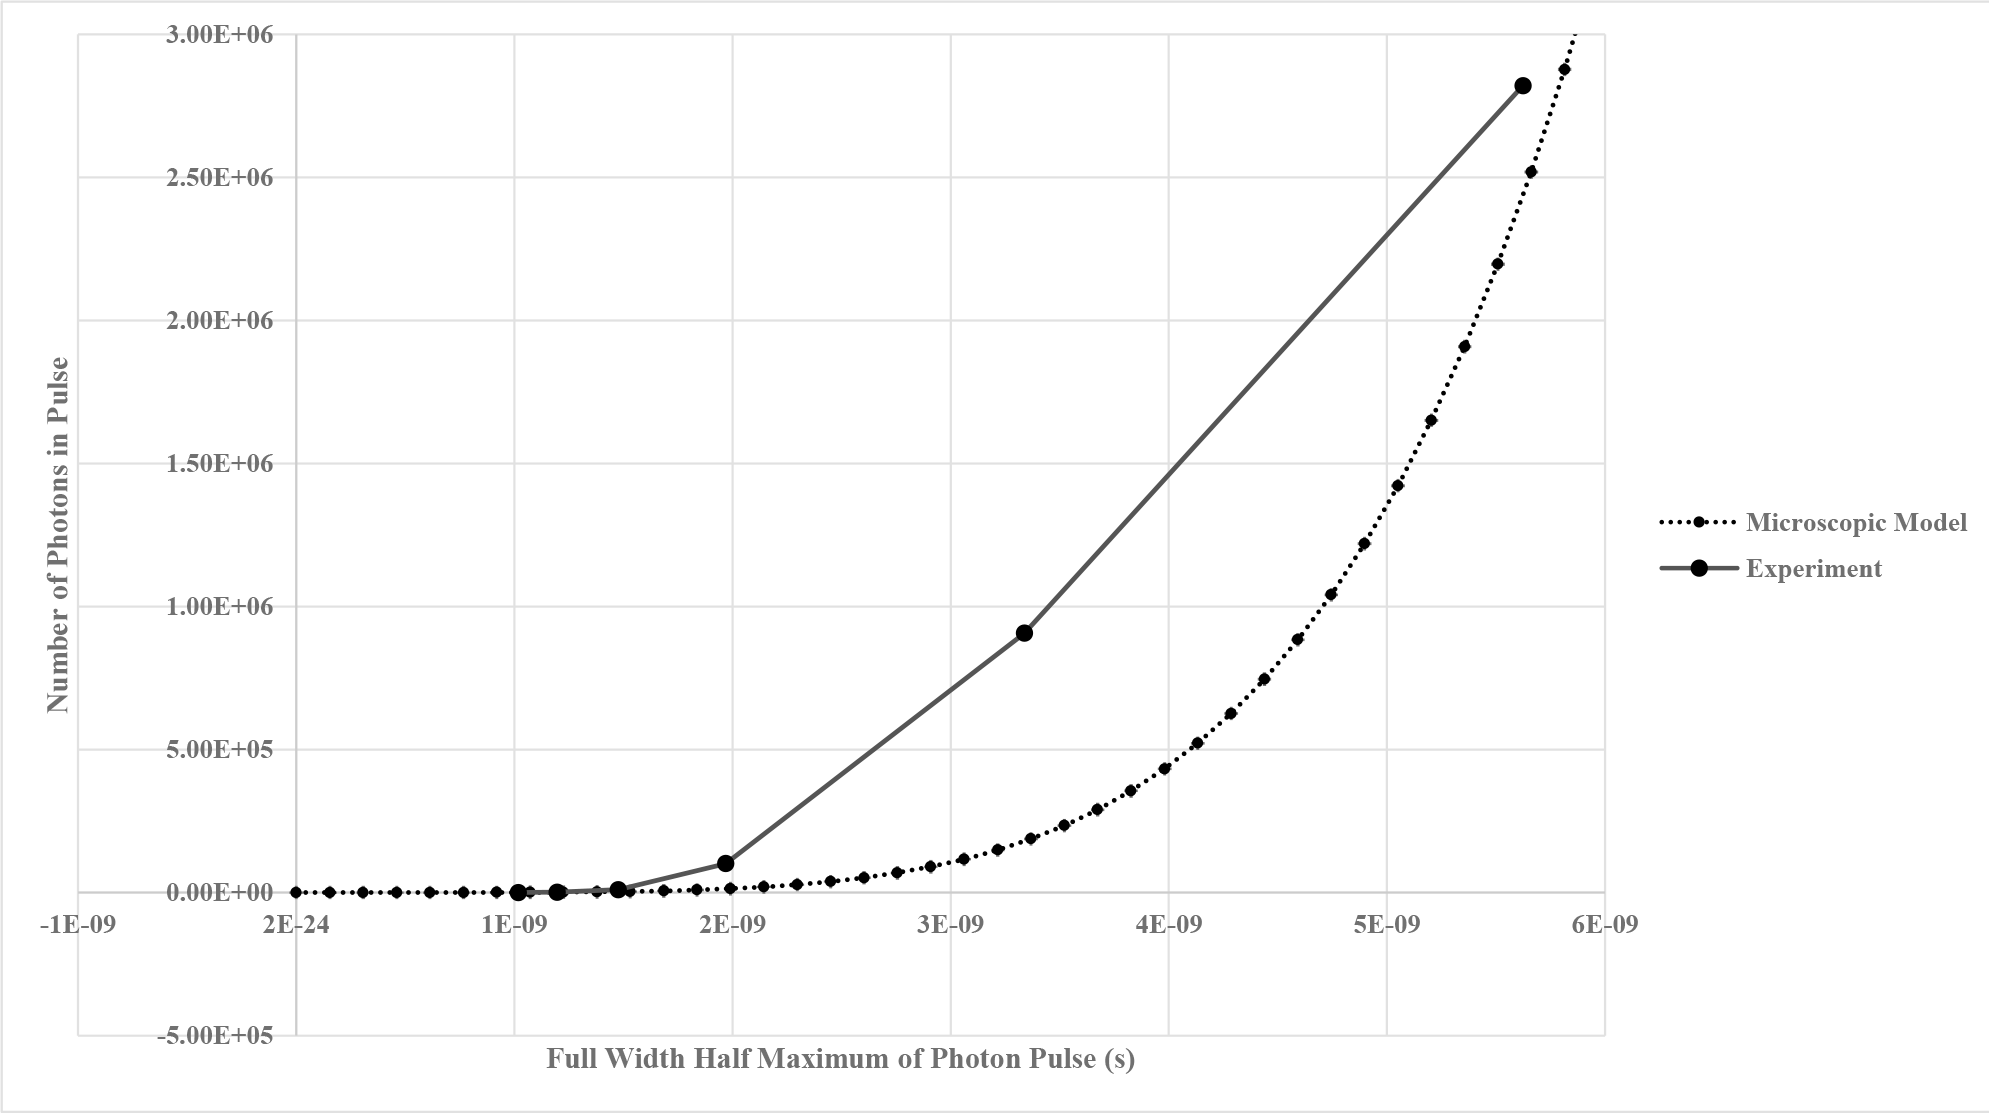
\includegraphics[scale=0.7]{Figures/MicroGraph}
	\caption{Data from Microscopic model with Experimental Data plotted alongside.\label{res:Mic:G1}}
\end{figure}
\begin{figure}[h]
	\centering
	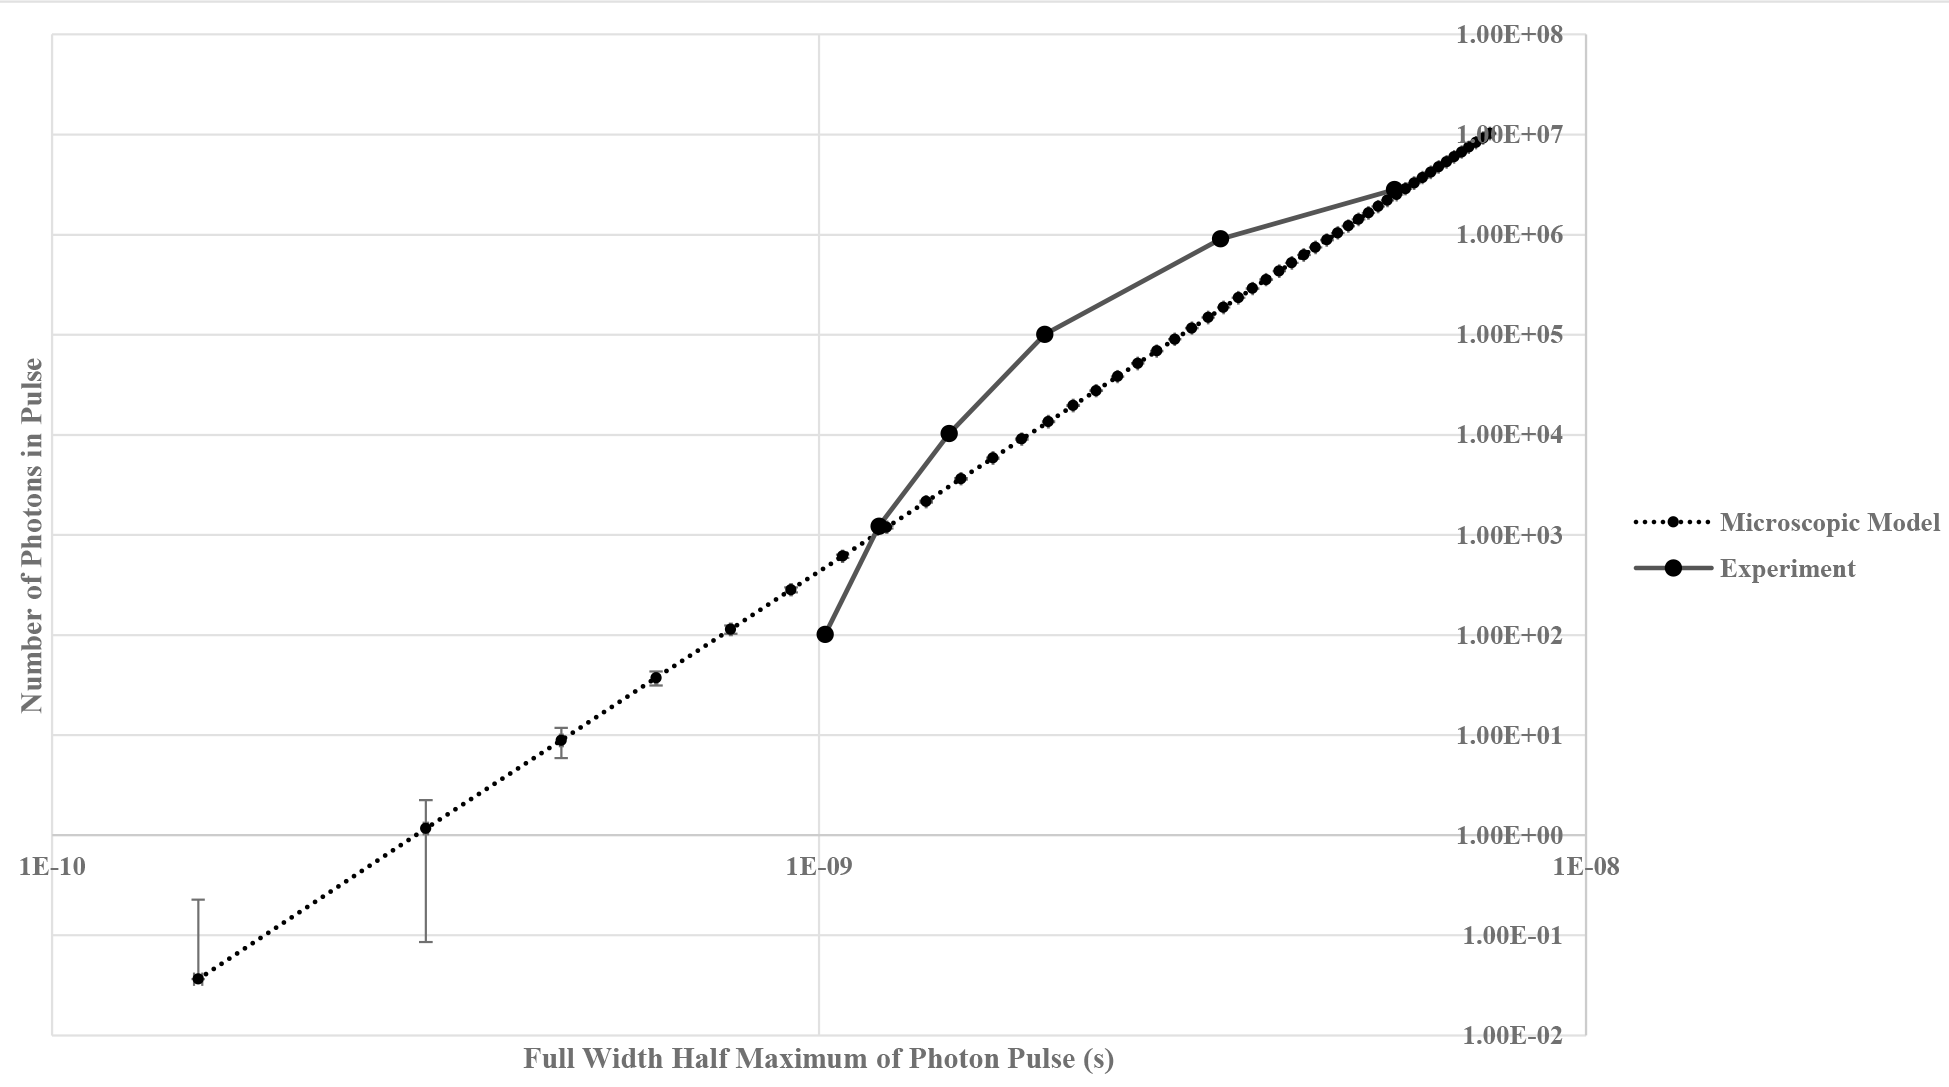
\includegraphics[scale=0.7]{Figures/MicroGraph_log}
	\caption{Log-log plot of Microscopic model data.\label{res:Mic:G1_log}}
\end{figure}
\bigskip

\subsection{Macro Simulation}


























\section{Discussion}
In this section, the results of the modelling compared to real-world results will be discussed. Topics of interest will be: Does the model predict the $N_{\gamma} \propto t^{3} $ results instead of the linear response predicted by Windisch's instantaneous current model ( $N_{\gamma} \propto t^{2} $) or does it manage the closer to experimental result of $t^{4}$?\\
Discuss the model's simulated capacitance and whether it's similar to that measured experimentally, or predicted by \textbf{Veledar}.\\
Did the model produce any temperature dependency graphs for photon emission, and if so, how do they again compare to experimental results?

\section{Conclusion}
In this section talk about the limits of the model (only 1D, inaccuracies with reality, etc) and discuss known ways to improve it. Discuss reasons for them not already being implemented (lack of knowledge about device[read: band structure, dimension, composition], more accurate models much more time consuming to build, etc...) \\


\section{References}
Format requested: "Last name, First initial. (Year published). Article title. Journal, Volume (Issue)" \textbf{How do I get it in that form $\downarrow$ ?} \textbf{Im aware a couple of these haven't worked properly from Bibtex, I'll find a fix later.}
\bibliography{thesis_ref}{}
\bibliographystyle{ieeetr}
\newpage

\section{Appendix}
The following sections detail an overview of the most important segments of code and its functionality. The complete source code for the project can be found online at \url{https://github.com/donmegamuffin/Thesis}.\footnote{As of writing on 24/03/2018.} Much of the following code has had comments removed or has been slightly altered for clarity within the code snippets.
\subsection{Code Overview: General}
The following subsections are the explanations of general code used across both simulations.
\subsubsection{FWHM calculation methods}
The calculation of the FWHM is split across 4 methods for readability and reuse. The algorithm for finding the FWHM is found in algorithm \ref{alg:Mac:FWHM}. Each step is handled by a separate method. \\ 
The first method simply handles finding the peak value of all the bins of a std::vector array, and returns its index:
\begin{lstlisting}[caption = Method for finding histogram peak bin]
int Device_1D::findPeakBin(std::vector<double> RadVector)
{
	double PeakValue = 0;
	int PeakValueAssociatedIndex = 0;
	for (std::size_t i = 0; i < RadVector.size(); i++)
	{
		if (RadVector[i] > PeakValue)
		{
			PeakValue = RadVector[i];
			PeakValueAssociatedIndex = i;
		}
	}
	return PeakValueAssociatedIndex;
}
\end{lstlisting}
It simply takes in a general vector of values (with the assumption the bins follow a single-peak curve), and iterates through each value, checks if it's higher than the current maximum value, and if so, sets the new peak value and associated index. It finally returns the peak with the maximum value.\\
To find the width of the curve, finding the points at which curve reaches half the peak is necessary. However, as the array is discrete, this has to be approximated to the nearest bin, giving the error on this value a maximum of $\pm 2\cdot t_{step}$, because each bin is calculated over a single time step.\\
 This is handled by the following two functions that have similar functionality. The first one finds the bin that falls below the half maximum, by starting at the peak value index in the vector, and working backwards:
\begin{lstlisting}[caption = Method for finding first bin to fall below half peak before peak]
int Device_1D::FWHMfindFirstBinBelow(std::vector<double> RadVector, 
				int PeakIndex)
{
	int Index = 0;
	for (std::size_t i = PeakIndex; i >= 0; i--)
	{
		if (RadVector[i] < (RadVector[PeakIndex] / 2))
		{
			Index = i;
			break;
		}
	}
	return Index;
}
\end{lstlisting}
The second method does the same, but finding the first bin after the peak, starting from the peak and incrementing the bin index until it's found.
\begin{lstlisting}[caption = Method for finding first bin to fall below half peak after peak]
int Device_1D::FWHMfindFirstBinAbove(std::vector<double> RadVector, 
				int PeakIndex)
{
	int Index = 0;
	for (std::size_t i = PeakIndex; i < RadVector.size(); i++)
	{
		if (RadVector[i] < (RadVector[PeakIndex] / 2))
		{
			Index = i;
			break;
		}
	}
	return Index;
}
\end{lstlisting}
This function puts the previous functions together to find the photon emission pulse bin's FWHM indices, and calculates the time by finding the bin's associated times by using its associated time vector:
\begin{lstlisting}[caption = Method for calculating FWHM from an std::vector of values]
double Device_1D::calculateFWHM(std::vector<double> RadVector,
				 std::vector<double> TimeVector)
{
	//Get the peak of the curve
	int PeakBin = findPeakBin(RadVector);
	//Get the first bin below half max
	int LowBin = FWHMfindFirstBinBelow(RadVector, PeakBin);
	//Get the first bin after half max
	int HighBin = FWHMfindFirstBinAbove(RadVector, PeakBin);
	//Return the difference in time between the associated time vector bins
	return (TimeVector[HighBin] - TimeVector[LowBin]);
}
\end{lstlisting}
These functions are implemented in both simulations as the method for finding FWHM of the photon pulses.

\subsubsection{External Voltage ramp up/down}
Both simulations have the same implementation for the calculation for the external voltage being applied to the device. It applies the tent-map implementation of external voltage ramp up and down with the equation:
\begin{eqnarray}
V(t) = \begin{cases}
\alpha t &t < t_{trans}\\
\alpha(2t_{trans} - t) &t \geq t_{trans}\\
\end{cases}
\end{eqnarray}
As parameters, it takes both the time the simulation is at (\textit{time}) and the point at which the simulation's voltage changes from ramp-up to ramp-down (\textit{transition\_time}), and returns the value $V(t)$ at that point.
\begin{lstlisting}
double Device_1D::inputV(double time, double transition_time)
{
	const double Vramp = 4e9;
	if (time < transition_time)
	return Vramp * time;
	else
	return Vramp * ((2 * transition_time) - time);
}
\end{lstlisting} 
The constant on line 3 is taken from experimental apparatus and was $\approx4\cdot10^9 Vs^{-1}$. The two return statements on line 5 and 7 are simply the function before and after the transition time.


\subsection{Code Overview: Micro}
The following subsections are the explanations of code used within the microscopic, segmented simulation.
\subsubsection{Current density calculation methods}
\begin{figure}[h]
	\centering
	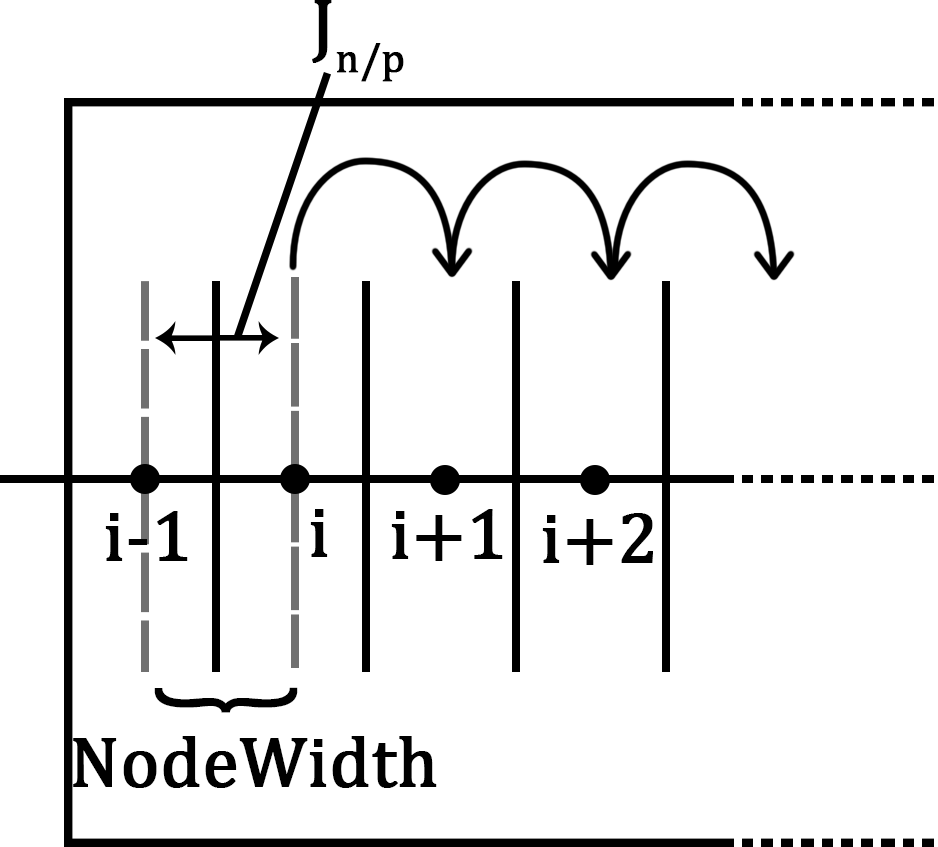
\includegraphics[scale=0.2]{Figures/JnL}
	\caption{\label{fig:Mic:JnL} Diagram of calculateJnLEC method's functionality.}
\end{figure}
This section contains the information on how current was calculated within the device.\\ Four functions were written, all with very similar structures but with alterations dependent on whether the order was starting from the left, or from the right, and whether it was done for the holes or electrons: JnL, JnR, JpL, and JpR. \\
For this example, JnL will be used to demonstrate the structure, with its depiction shown in Figure \ref{fig:Mic:JnL}.
The code worked by taking the device's std::vector<Node>s and manipulating the electron (or hole) densities by applying:
\begin{eqnarray}
	&J_n = -q\mu_n n\nabla V + \mu_n n \nabla E_c + q D_n \nabla n\\
		\hookrightarrow &J_n = -q\mu_n(\dfrac{n_{i+1}+n_{i}}{2})(\dfrac{V_{i+1}-V_{i}}{a})\\
	+& \mu_n (\dfrac{n_{i+1}+n_{i}}{2})(\dfrac{E_{c(i+1)}-E_{c(i)}}{a}) + qD_n(\dfrac{n_{i+1}-n_{i}}{a}) \\
\end{eqnarray}
starting from the second node, to the last in that order, calculating the current between the node, and the that of the one to its left.\\
Line 3 creates a variable to store the absolute value of the current between the two nodes and adds it to a cumulative value to be returned once the function is complete. This return is used in parts of the program to guage whether the device is in equilibrium or not.\\
Lines 11 and 12 simply find the current and transfer the difference from one to other with correct dependence depending on the direction of the current density.\\
The exchange scale multiplies this transfer which results in significantly fewer loops required where time is not a factor in the calculation. As current density is charge transfer per unit time, it also works as a crude method of integrating the current calculation over a time period, treating it as constant current.\\
By using this approximation method, it is only valid for relatively small approximations where $J_{nL} t \ll n$ and is the equivalent of doing:
\begin{equation}
 \sum\limits_{i=1}^{x}\dfrac{dn}{dt}\Big|_{t=t_i} = \lim\limits_{n''(t)\to 0} x\cdot \dfrac{dn}{dt}\Big|_{t=t_1}  
\end{equation}
and is assumed that the rate in change in current transfer is smooth and small as to allow for this approximation. Because, in this approximation, $\frac{dn}{dt}$ is only needed to be calculated once, this is far faster for use in the equilibrium code by applying an approximation factor.
\begin{lstlisting}[caption = Example of the current calculation algorithm]
double Device_1D::calculateJnLEC(double exchangeScale)
{
	double JnL_cum = 0;	
	for (std::size_t i = 1; i < nAry.size(); i++)
	{
		double dn = (nAry[i].n - nAry[i - 1].n) / nodeWidth;
		double dV = (nAry[i].V - nAry[i - 1].V) / nodeWidth;
		double dEc = (nAry[i].Ec - nAry[i - 1].Ev) / nodeWidth;
		double n = (nAry[i].n + nAry[i - 1].n) / 2;
		double JnL = (-q * mu*n*dV) - (mu*n*dEc) + (q*D*dn);
		nAry[i].n = nAry[i].n - (JnL*exchangeScale);
		nAry[i - 1].n = nAry[i - 1].n + (JnL*exchangeScale);
		JnL_cum += abs(JnL);
	}
	return JnL_cum;
}
\end{lstlisting}

\subsubsection{Voltage calculation method}
This consists of a single function which cycles through each of the nodes in the device and does the following calculation following from the derivation shown in section \ref{sec:Meth:Mic:eqn}:
\begin{eqnarray}
& \dfrac{V_{i+1}+V_{i-1}-2V_i}{a^2} = \dfrac{q}{\epsilon_r \epsilon_0}(p+N_D-n-N_A) \\
\hookrightarrow & V_i = \frac{1}{2}[\dfrac{q}{\epsilon_r \epsilon_0}(p+N_D-n-N_A) + V_{i+1}+V_{i-1}]
\end{eqnarray}
with the cap-ends of the device having slightly modified calculations, for first node of the device:
\begin{equation}
V_i = \frac{1}{2}[\dfrac{q}{\epsilon_r \epsilon_0}(p+N_D-n-N_A)] + V_{i+1} 
\end{equation}
and last node of the device:
\begin{equation}
V_i = \frac{1}{2}[\dfrac{q}{\epsilon_r \epsilon_0}(p+N_D-n-N_A)] + V_{i-1} 
\end{equation}
\begin{lstlisting}[caption = Voltage calculation method]
void Device_1D::calculateVoltages()
{
	//Loop through each of the nodes
	for (std::size_t i = 0; i < nAry.size(); i++)
	{
		double a2 = pow(nodeWidth, 2);
		double C = (q*a2) / e_0;
		double netCharge = nAry[i].p + nAry[i].Nd - nAry[i].n - nAry[i].Na;
		//If node is at a cap position change calculation
		if (i == 0)
		{
			nAry[i].V = (C*(netCharge)+ nAry[i + 1].V);
		}
		else if (i == (nAry.size() - 1))
		{
			nAry[i].V = (C*(netCharge)+nAry[i - 1].V);
		}
		else	//Do normal calculation
		{
			nAry[i].V = 0.5*(C*(netCharge)+nAry[i - 1].V + nAry[i + 1].V);
		}
	}
}
\end{lstlisting}
\medskip
The first \textbf{if} statement implement the calculation if it's doing it for the first node, and the \textbf{else if} statement implements the end-node calculation. The first lines of the for loop are there to break down the calculation's constants for a node and make later calculations more readable. 

\subsubsection{Charge injection Method}
\begin{figure}[h]
	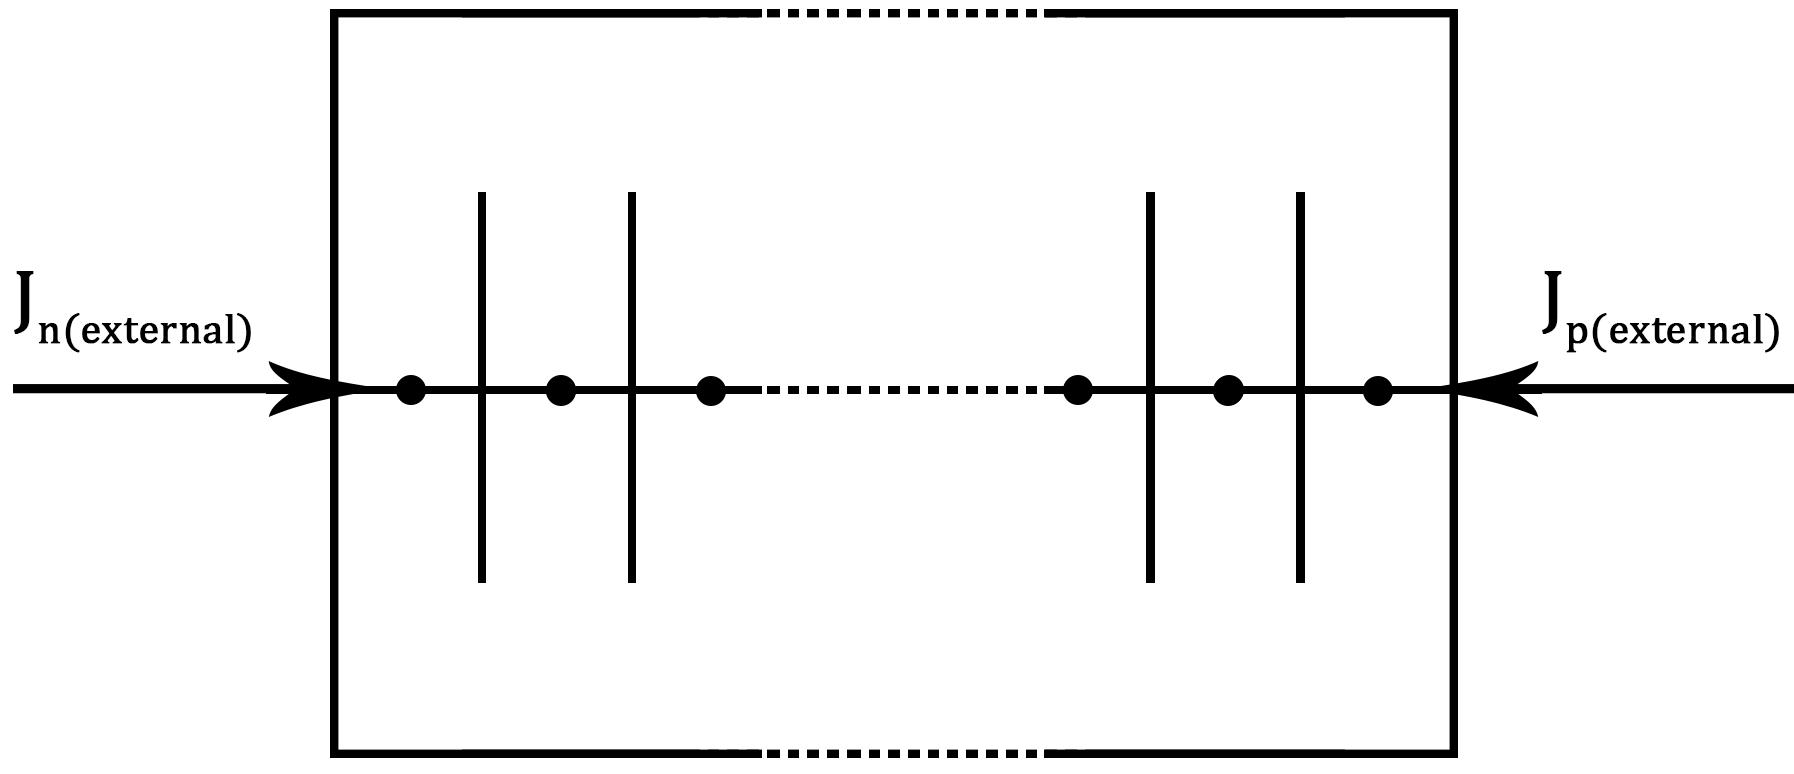
\includegraphics[scale=0.17]{Figures/Injection}
	\caption{\label{fig:Code:Injection} Visualisation of charge injection method}
\end{figure}
This method handles the injection of charges at the end nodes of the device. A visualisation of what the code is doing can be seen in figure \ref{fig:Code:Injection} and simply injects these charges into the end nodes of the device.
It has two parameters: Current density ($J_{external}$) and the Injection Duration (using the $t_{step}$ for the simulation). The total density of charges to be added to the ends in a single time step of the device will simply be $\frac{dn}{dt} = J_{external}\cdot t$.\\
The $J_{external}$ used in the parameter for the simulation is the current density calculated assuming Ohm's Law is correct:
\begin{equation}
	J = \frac{I}{A} = \frac{V}{A\cdot R}
\end{equation}
\begin{lstlisting}[caption = Charge injection method, basicstyle=\tiny]
void Device_1D::injectCharges(double CurrentDensity, double injectionDuration)
{
	//Inject n in left, p on right.
	nAry[0].n += (CurrentDensity*injectionDuration);
	nAry[nAry.size() - 1].p += (CurrentDensity*injectionDuration);
	return;
}
\end{lstlisting}

\subsubsection{Simulation inner loop method}
This section covers the details of how the inner loop is handled. There are two \textit{overloads} for this function but it will be demonstrated with the variant used for the full simulation rather than the single-use simulation which has minor changes (e.g. outputs a full Debug file of all the data, etc.).\\
It requires references to two external \textbf{double} values as Output parameters to pass data calculated within this inner loop for both the FWHM and total photons calculated by the simulation. The last two parameters are the simulation step time and the time the voltage transitions from ramping up to ramping down.
\begin{lstlisting}
void Device_1D::simulateDevice(double & outFWHM, 
			double & outRrad, double t_step, double t_trans)
{
	double t_now = 0;	//current device simulation time
	std::vector<double> t_Vec;	//Stores all the times
	double Rrad_now;		//Single Loop number of photons
	std::vector<double> Rrad_Vec;	//Current device radiation
	double Rrad_cum = 0;	//Cumulative radiation
	double inV = 0;			//Input voltage
	double J = 0;			//J
	
	//Main function loop
	do
	{
		t_now += t_step;
		t_Vec.emplace_back(t_now);
		
		inV = inputV(t_now, t_trans);
		J = inV / (A * R);
		
		injectCharges(J, t_step);
		calculateVoltages();
		calculateJpREV(t_step);
		calculateJnLEC(t_step);
		
		Rrad_now = calcRadRecombine(t_step);
		Rrad_Vec.emplace_back(Rrad_now);
		Rrad_cum += Rrad_now;
	} while (Rrad_now>0);
	
	outFWHM = GetRadFWHM(Rrad_Vec, t_Vec);
	outRrad = Rrad_cum;
}
\end{lstlisting}
The simulation is contained in a \textbf{do....while} function as to allow it to run always run a single time, and then loop as long as the Radiative recombination is above zero, automatically terminating the loop once all photons have been emitted. This way of doing it meant that it works universally for any length of transition time.\\
In line 18, the "inputV(...)" function, is the function used to calculate the voltage at a point in time, calculated from the tent map discussed in section \ref{sec:Meth:Mic:eqn} which returns the external Voltage applied.
The following lines calculate the external current, inject the charges, and then calculate the internal current. \\
Line 26 calculates the radiative recombination across every node using: 
\begin{equation}
	R_{rad} = Bnp\cdot t_{step}
\end{equation}
where $R_{rad}$ is the number of photons emitted during the simulation time-step, which is then put at the end of a Vector to be stored (so it can be user later to output to file in the other overload) and then added to the total cumulative photons in line 28.\\
At the end of the simulation loop, the FWHM is calculated in line 31 and passed to the Output parameter \textit{outFWHM} and the cumulative number of photons passed to \textit{outRad}.\\

\subsubsection{Full ranged simulation (outer loop) method}
The following code is the full implementation of the algorithm \ref{alg:Mic:Outer} found in section \ref{sec:Mic:FullSim}. Lines 5 to 10 hold data for later use, whilst lines 16 to 28 are the actual implementation of the algorithm with 26 ad 27 putting the FWHM and associated cumulative photon counts of the loop onto the data storage std::vectors in 6 and 7. These two std::vectors are then written to a .csv file through lines 30 onwards and then closing the file at the end.
\begin{lstlisting}[caption = Full outer simulation loop method]
void Device_1D::fullSim(std::string eqmFileName, 
					double timeStep, double transStep, double transMax)
{
	//Simulation Data arrays for output
	std::vector<double> t_trans_Vec;
	std::vector<double> FWHM_Vec;
	std::vector<double> Rcum_Vec;
	
	double FWHM_now = 0;	//Holds the loop FWHM
	double Rcum_now = 0;	//Holds the loop Rcum
	
	//Open filestream for printing results
	std::ofstream resultsFile;
	resultsFile.open(eqmFileName + "_Rad_results.csv",'w');
	
	for (int i = 0; i*transStep < transMax; i++)
	{
		//Set up device
		loadState(eqmFileName);
		
		//Add the transition time to trans vector
		t_trans_Vec.emplace_back(i*transStep);
		
		simulateDevice(FWHM_now, Rcum_now, timeStep, i*transStep);
		
		FWHM_Vec.emplace_back(FWHM_now);
		Rcum_Vec.emplace_back(Rcum_now);
	}
	//Print Results to file
	for (auto a : t_trans_Vec)
	{
		resultsFile << a << ",";
	}
	resultsFile << std::endl;
	for (auto a : FWHM_Vec)
	{
		resultsFile << a << ",";
	}
	resultsFile << std::endl;
	for (auto a : Rcum_Vec)
	{
		resultsFile << a << ",";
	}
	resultsFile << std::endl;
	
	resultsFile.close();
}
\end{lstlisting}

\subsubsection{Equilibrium method}
The following code is used for bringing a loaded device to equilibrium. It follows the principles of algorithm \ref{alg:mic:Eqm} in section \ref{sec:Mic:Eqm}. \\
As parameters it takes the a user-defined "Tolerance", an "exchange scale" (approximation factor), an output stream to write to a file, and a bool for defining whether it should write to console or not.\\
The "Tolerance" value is used in two ways: first to define what is considered "equilibrium" in terms of total current density maximum across the device, and as the point at which the simulation may reach convergence in the case it never goes below tolerance value. This is done on line 8, where the first part of the \textbf{if} statement checks for the first condition, and the second part checks the previous loop's total current isn't closer than a limit (of $0.1\cdot Tolerance$)to the current loop's. Lines 4 and 5 are used to hold those two loop total current densities. \\
\begin{lstlisting}
void Device_1D::bringToEqm(double Tolerance, double exchangeScale, 
std::ostream &fileOutput, bool bPrintConsole)
{
	double Jtot = 1e13;
	double J_prev = 1e8;
	//Whilst the current is higher than the current equilibrium limit
	//Loop until Jtot is below user defined limit
	while (Jtot > Tolerance && abs(Jtot - J_prev)>(0.1*Tolerance))
	{
		J_prev = Jtot;	
		Jtot = calculateJnREC(exchangeScale) + calculateJpLEV(exchangeScale);
		calculateVoltages();
		cancelCharges();
		//OPTIONAL : Print the current found to console
		if (bPrintConsole) 
		{	
			std::cout << "\r" << Jtot << "                 ";
		}
		//Print current to file
		fileOutput << Jtot << std::endl;
	}
	if (bPrintConsole) { std::cout << "\n Equilibrium calculation finished." << std::endl; }
	return;
}
\end{lstlisting}
Lines 15 to 18 and line 22 only run if the bool in the parameter is set to true, and simply keeps the user up to date in the console.

\end{document}
